\documentclass[UTF8]{article}
\usepackage{bm}
\usepackage{amsmath}
\usepackage{cases}
\usepackage{cite}
\usepackage{graphicx}
\usepackage[margin=1in]{geometry}
\geometry{a4paper}
\usepackage{fancyhdr}
\pagestyle{fancy}
\usepackage{wrapfig}
\fancyhf{}
\usepackage{float}  %设置图片浮动位置的宏包
\usepackage{subfigure}
\usepackage{caption}
\usepackage{booktabs}
\usepackage{listings}
\usepackage{xcolor}
\usepackage{multirow}
\lstset{numbers=left, %设置行号位置
	numberstyle=\tiny, %设置行号大小
	keywordstyle=\color{blue}, %设置关键字颜色
	commentstyle=\color[cmyk]{1,0,1,0}, %设置注释颜色
	frame=single, %设置边框格式
	escapeinside=``, %逃逸字符(1左面的键),用于显示中文
	breaklines, %自动折行
	extendedchars=false, %解决代码跨页时,章节标题,页眉等汉字不显示的问题
	xleftmargin=2em,xrightmargin=2em, aboveskip=1em, %设置边距
	tabsize=4, %设置tab空格数
	showspaces=false %不显示空格
}

\title{The Frank Hertz \& Metal fugitive work experiment}
\author{by 22 Artificial Intelligence ChenxuZhang}
\date{2023.5.23}
\pagenumbering{arabic}

\begin{document}
	
	\fancyhead[L]{ChenxuZhang}
	\fancyhead[R]{ID 202264691028}
	\fancyfoot[C]{\thepage}
	
	\maketitle
	\tableofcontents
	\newpage
	
	\section{Abstract}
\subsection{The Frank Hertz Experiment}
In 1913 the Danish physicist Bohr, based on Rutherford's model of the atomic nucleus, combined with Planck's quantum theory to propose the concept of atomic energy level and established the atomic model theory, which successfully explained the stability of the atom and the line spectrum of the atom. The theory states that an atom does not radiate energy when it is in a stable state, and it radiates energy when it jumps from a higher energy state (energy) to a lower energy state (energy), which satisfies $\bigtriangleup E=E_m-E_n$. For the energy provided by the outside world, the atom absorbs and leaps only if it satisfies the energy level difference of the leap to the higher energy level, otherwise it does not.

1914 German physicists Frank and Hertz determined the first excitation potential of the mercury atom using an experiment with slow electrons passing through the mercury vapor, thus proving the existence of discrete energy states of the atom. Later they observed the light radiated by the excited atoms in the experiment when they returned to the normal state, and the measured frequencies of the radiated light satisfied the Bohr theory well. The results of the Frank Hertz experiment provided direct evidence for the Bohr theory. Bohr was awarded the 1922 Nobel Prize in Physics for his theory of the atomic model, and the Frank-Hertz experiment was awarded the Nobel Prize in Physics in 1925.
 \subsection{Metal fugitive work experiment}
There are a large number of free electrons in metals, but the energy of electrons inside the metal is lower than the energy outside, so a certain amount of energy is needed to provide electrons when they escape from the metal, and this energy is called electron escape work. The work of escape (work function) is one of the basic properties of metallic materials.

Metal fugitive work is an important parameter in the study or technology of electronic devices, such as light-emitting diodes (LED) and solar cells. The study of physical properties such as the fugitive work of metallic materials can not only improve the application of metallic materials in electronics, but also deepen the understanding of microscopic atomic structure, especially it is important to revise the relevant atomic structure theory and calculation methods.
	
\section{Purpose of the experiment}
	\subsection{The Frank Hertz Experiment}
   $\bm{A}$.To learn how to measure the first excitation potential of an atom.\\
   $\bm{B}$.To confirm experimentally the existence of atomic energy levels.\\
   $\bm{C}$.To study the factors affecting the anode current of inflatable electron tubes and to analyse the mechanism.
   
   \subsection{Metal fugitive work experiment}
      $\bm{A}$.Determine the electron escape work of tungsten metal using the Richardson linear method.\\
      $\bm{B}$.Learn how to process data.\\

	\section{Experimental apparatus}
	For the above experiments we will use the same essentially identical experimental equipment for the measurements, as follows:
	
	Electronic tube comprehensive experimental instrument:
		\begin{figure}[H]
	\centering
	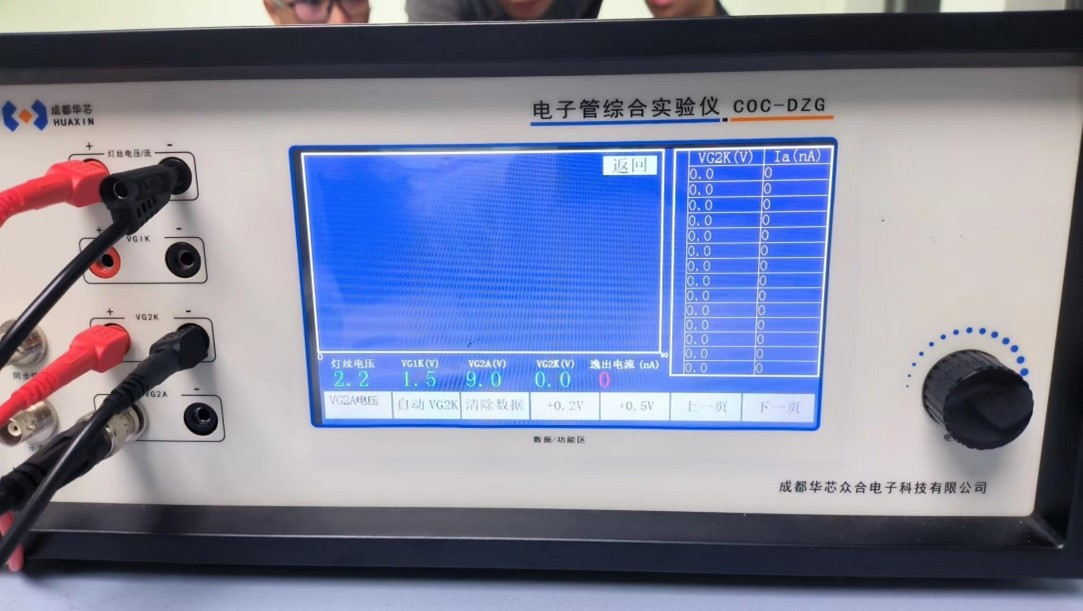
\includegraphics[clip,scale=0.8,trim={0 0 0 0}]{fig/fig1.jpg}
    \caption{Electronic tube comprehensive experimental instrument}
    \label{figure.1}
        \end{figure} 
        
    Electronic tube comprehensive experiment instrumen:
    		\begin{figure}[H]
    	\centering
    	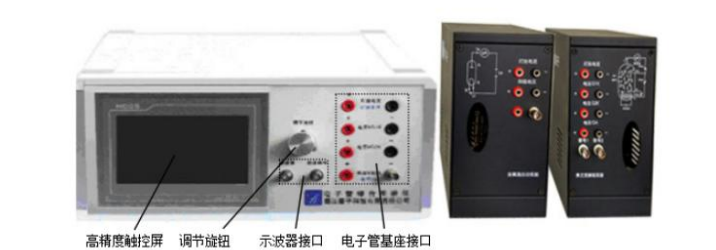
\includegraphics[clip,scale=1,trim={0 0 0 0}]{fig/fig2.png}
        \caption{Electronic tube comprehensive experiment instrument}
        \label{figure.2}
            \end{figure} 
            
    \begin{itemize}
      \item The electron tube: The electron tube is one of the core components of the experimental instrument. It is a vacuum tube that contains components such as cathode, anode, and grid. The structure and parameters of the electron tube can be selected and adjusted according to the experimental requirements.
      
      \item Power supply: Electron tube experimental instruments are usually equipped with a stable and adjustable DC power supply to provide the necessary voltage and current for the electron tube. This allows for the adjustment of the operating point of the electron tube to observe and record performance changes under different parameters.
      
      \item Measurement instruments: The instrument also includes various measurement instruments to accurately measure the performance parameters of the electron tube. For example, voltmeters and ammeters can be used to measure voltage and current values, while an oscilloscope can display and record the output signals of the electron tube.
      
      \item Control panel: Electron tube comprehensive experimental instruments are typically equipped with an integrated control panel for controlling experimental parameters and observing experimental results. The control panel may include knobs, switches, and indicator lights to facilitate operation and monitoring by researchers.
      
      \item Connection interfaces: To facilitate experiments and data recording, electron tube comprehensive experimental instruments usually provide various connection interfaces. These interfaces can be used to connect external devices such as computers or data acquisition systems for data analysis and recording.
    \end{itemize}
    
        
	\section{Experimental principles}   
	\subsection{The Frank Hertz Experiment}
	According to Bohr's atomic theory, atoms can only stay in stable states, called "stationary states," for a relatively long time. Atoms in stationary states neither emit nor absorb energy, and the energy of each stationary state is discrete, meaning that they are at different energy levels. Atoms can only absorb or radiate energy equivalent to the energy difference between the energy levels. When an atom transitions from one stationary state to another, energy emission and absorption occur, and the frequency of the emitted or absorbed energy radiation is also a constant value. The radiation frequency, denoted as $v$, is determined by the energy difference between the two levels,$hv = \bigtriangleup E=E_m-E_n$   and Planck's constant, $h$, such that 
	\begin{eqnarray}
	v = \frac{E_m-E_n}{h} 
	\end{eqnarray}
	
	To change the state of an atom, external energy must be applied to the atom to excite it and induce a transition. The Franck-Hertz experiment achieves changes in atomic energy states by accelerating electrons, which have a certain amount of energy, and colliding them with atoms to exchange energy.
	
	The principle of the Franck-Hertz experiment involves an argon-filled electron tube with a cathode $K$ , an anode $A$ , and two grids  $G_1$ and $G_2$  serving as the first and second grids, respectively.
	
	A positive voltage is applied between the cathode $K$ , grid $G_1$ , and grid $G_2$  to provide energy to the electrons. The role of $V_{G_{1}K}$  is primarily to eliminate the effect of space charge on cathode electron emission and to improve the emission efficiency. A reverse voltage   is applied between grid $G_2$  and the anode $A$ to create a repelling electric field.
	
	\begin{figure}[H]
        	\centering
        	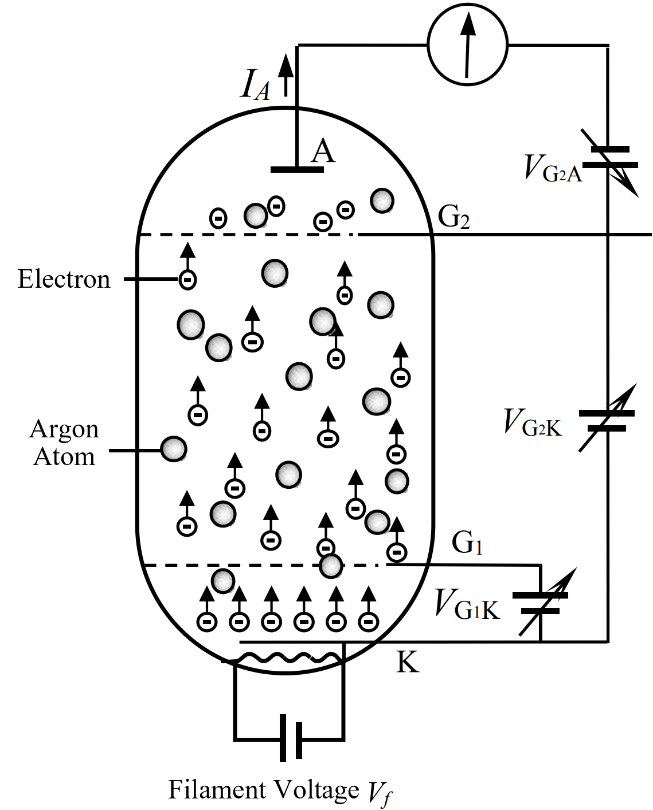
\includegraphics[clip,scale=1,trim={0 0 0 0}]{fig/fig3.png}
            \caption{Experimental schematic diagram}
            \label{figure.3}
   \end{figure} 
   
   The electrons are emitted from the hot cathode K and gain energy in the $K\sim G_2$ region, but lose energy in the $A\sim G_2$ region. If the kinetic energy of the electron is greater than or equal to the $eV_{G_2A}$  when it enters the $A\sim G_2$ region, it can reach the anode and form an anode current $I_A$ .
   
   In the $K\sim G_2$ interval, the electrons are rapidly accelerated by the electric field and gain energy. In the $G_1\sim G_2$ interval, the electrons continue to gain energy from the electric field and collide with argon atoms. When the electron's energy is less than the energy level difference between the first excited state and the ground state of the argon atom, i.e., $\bigtriangleup E = E_1-E_2$ , the argon atom basically does not absorb the energy of the electron, and the collision is elastic. When the electron's kinetic energy reaches $\bigtriangleup E$ , it may be absorbed by the argon atom during the collision, and the collision becomes inelastic. ΔE is called the critical energy. In the $A\sim G_2$ interval, the electrons overcome the repulsive electric field force and lose energy due to the work done. If the kinetic energy of the electron entering this interval is less than $eV_{G_2A}$ , it cannot reach the anode.
   
	\begin{figure}[H]
        	\centering
        	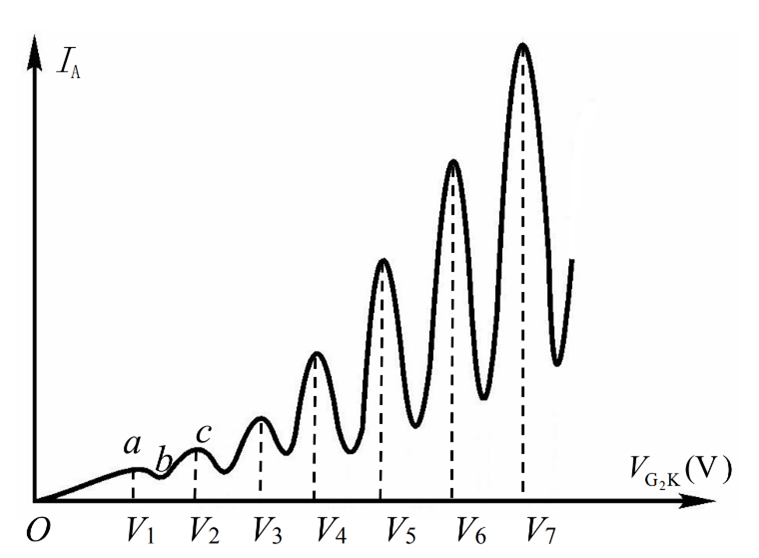
\includegraphics[clip,scale=1,trim={0 0 0 0}]{fig/fig4.png}
            \caption{Frank-Herts Experiment Curve}
            \label{figure.4}
   \end{figure}    
   
   Hence, after being accelerated from $K$ to $G_2$ , if $eV_{G_2A}< \bigtriangleup E$ , the electron enters the $A\sim G_2$ region with an energy of $eV_{G_2A}$. With the increase of $eV_{G_2A}$, more and more electrons have enough energy to overcome the repulsive field and reach the anode, and the current $I_A$  increases.
   
   Continuing to increase $V_{G_2A}$, the remaining energy of the electrons after collision also increases, and the number of electrons reaching the anode gradually increases. 
   
   When $eV_{G_2A}< n\bigtriangleup E$, the electrons may lose energy by colliding with argon atoms $n$ times before entering the $A\sim G_2$ region. The curve of the anode current  $I_A$ versus the acceleration voltage $eV_{G_2A}$ then forms $n$ peaks. Whenever 
   \begin{eqnarray}
   V_{G_2A}=nV_0
   \end{eqnarray}
   
   the anode current drops accordingly, and the voltage difference between adjacent peaks $V_0$ is called the first excitation potential of argon atoms. The energy difference between the first excited state and the ground state of argon atoms is 
   \begin{eqnarray}
   \bigtriangleup E = eV_0
   \end{eqnarray}
   
   \subsection{Metal fugitive work experiment}
   \subsubsection{Egress function}
   According to the theory of metallic electrons in solid state physics, the distribution of conduction electrons in metals follows the Fermi-Dirac distribution according to energy, i.e
   \begin{eqnarray}
   f(E)=\frac{d N}{d E}=\frac{4 \pi}{h^{3}}(2 m)^{\frac{3}{2}} E^{\frac{1}{2}}\left(e^{\frac{E-E_{F}}{k T}}+1\right)^{-1}
   \end{eqnarray}
   where EF is called Fermi energy level.
   
   At absolute zero, the energy distribution of the electron is shown in Figure 4.12-1, curve 1. The maximum energy possessed by the electron at this time is EF . The energy distribution of electrons when the temperature increases is shown in Figure 4.12-1, curve 2. The number of electrons with higher energy decreases exponentially with the increase in energy, where the few electrons with higher energy have higher energy than E.

	\begin{figure}[H]
        	\centering
        	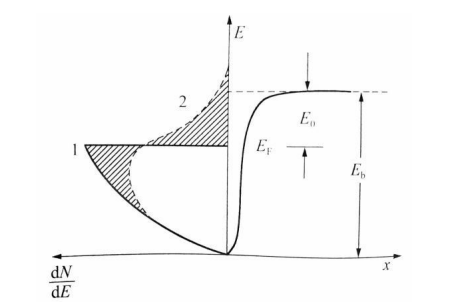
\includegraphics[clip,scale=1,trim={0 0 0 0}]{fig/fig5.png}
            \caption{Metal conduction electron energy distribution}
            \label{figure.5}
   \end{figure}    
   
   At absolute zero, the energy distribution of the electron is shown in Figure 4.12-1, curve 1. The maximum energy possessed by the electron at this time is EF . The energy distribution of electrons when the temperature increases is shown in Figure 4.12-1, curve 2. The number of electrons with higher energy decreases exponentially with the increase in energy, where the few electrons with higher energy have higher energy than E. 
   
   Normally, since there is a potential barrier E between the surface of the metal and the outside world (vacuum), electrons must have at least energy E to escape from the surface of the metal. As can be seen from the figure, the minimum energy required for an electron to escape from a metal at absolute zero is
   \begin{eqnarray}
   W=E_{b}-E_{F}=e \varphi
   \end{eqnarray}
   $W (or e\varphi)$ is called the work of escape of metal electrons, and its common unit is electron volt $(eV)$, which characterizes the energy required to give the maximum energy of electrons escaping from the metal surface in the metal at absolute zero. φ is called the escape potential, and its value is equal to the size of the work of escape of electrons in electron volts.
   
   \subsubsection{Thermoelectric emission circuit}
   
   The cathode of the vacuum diode (made of tungsten wire of the metal under test) is heated by  current to raise the pole temperature, and the increase in temperature changes the energy distribution of electrons within the tungsten wire, so that the number of electrons with kinetic energy greater than E increases and the number of electrons with kinetic energy greater than reaches an observable size, so that the number of hot electrons emitted from the metal surface reaches a detectable number.
   	\begin{figure}[H]
           	\centering
           	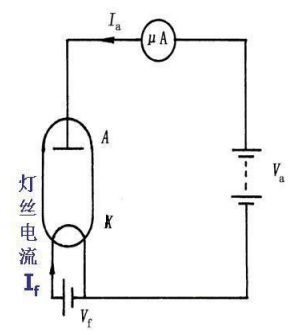
\includegraphics[clip,scale=1,trim={0 0 0 0}]{fig/fig6.png}
               \caption{Schematic}
               \label{figure.6}
      \end{figure} 
   Therefore, when no positive voltage is applied to the anode A (=0 in the figure), a thermal
   emission current I (called zero-field current) will also be detected in the external circuit
   connecting the two electrodes.
   
   \subsubsection{Richardson Linear Method}
   The above zero-field current strength I is determined by the Richardson-Ressiman formula, with:
   \begin{eqnarray}
   I=A S T e^{-\frac{e \varphi}{k T}}
   \end{eqnarray}
   here $A$ is the coefficient related to the chemical purity of the cathode surface  $S$ is the effective emitting area of the cathode , $T$ is the absolute temperature ofthe cathode emitting hot electrons (in K), and k is the Boltzmann constant. It is the basic principle equation for measuring electron escape work by hot electron emission. This equation shows that the electron escape work $( e\varphi )$ plays a decisive role in the intensity of hot electron emission. Dividing both sides of the equation and taking the logarithm, we get:
   \begin{eqnarray}
   \lg \frac{I}{T^{2}}=\lg A S-\frac{e \varphi}{2.30 k T}=\lg A S-5.04 \times 10^{3} \varphi \frac{1}{T}
   \end{eqnarray}
   
   This equation shows that $\lg \frac{I}{T^{2}}$ is linearly related to $\frac{1}{T}$ If $\lg \frac{I}{T^{2}}$  is the vertical coordinate and $\frac{1}{T}$  is the horizontal coordinate, the slope of the line can be used to find the electron escape potential $\varphi$ and the electron escape work $e\varphi$. Such a mathematical treatment is called Richardson's linear method.
   
   \subsubsection{Measurement of zero-field current I}
   Space charge is formed during the continuous flight of hot electrons from the cathode to the anode. The electric field of the space charge prevents the subsequent electrons from flying tothe anode. This seriously affects the measurement of the zero-field current. In order to overcome the influence of the space charge electric field, so that the electrons can quickly fly to the anode once they escape, an accelerating field has to be added between the anode and the cathode, but the presence of �� will produce the Schottky effect, so that the potential barrier on the cathode surface is lowered, the electron escape work is reduced, and the emission current becomes larger, so the measured current is the emission currenton the cathode surface under the action of the accelerating electric field, instead of the zero-field current I.
      	\begin{figure}[H]
              	\centering
              	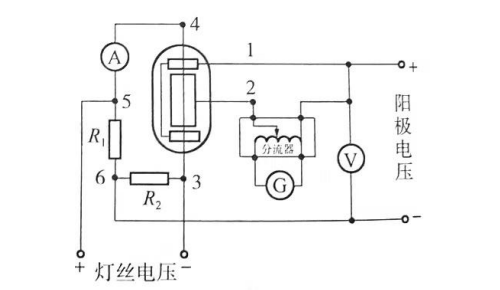
\includegraphics[clip,scale=1,trim={0 0 0 0}]{fig/fig7.png}
                  \caption{Experimental circuit diagram}
                  \label{figure.7}
         \end{figure} 
         
   It can be shown that the zero-field currents $I$ and $I_a$ are related as:
   \begin{eqnarray}
   I_{a} & =I \exp \left(\frac{0.439 \sqrt{E_{a}}}{T}\right)
   \end{eqnarray}
   
   Taking the logarithm of the above equation and taking the curve straight, we have:
   \begin{eqnarray}
   \lg I_{a} & =\lg I+\frac{0.439 \sqrt{E_{a}}}{2.30 T}
   \end{eqnarray}
   
   Usually the cathode and anode into a co-axial cylindrical shape, ignoring the contact potential
   difference and other effects, the cathode surface $U$. The accelerated electric field can be
   expressed as $E_{a}=\frac{U_{a}}{r_{1} \ln \left(r_{2} / r_{1}\right)}$   , where $r_1$ and $r_2$ are the radii of the cathode and anode, respectively, and $U_a$ is the anode voltage. Substitute $E_a$ into the above equation to get:
   \begin{eqnarray}
   \lg I_{a} & =\lg I+\frac{0.439}{2.30 T} \frac{1}{\sqrt{r_{1} \ln \left(r_{2} / r_{1}\right)}} \sqrt{U_{a}}
   \end{eqnarray}
   
   This equation is the basic formula for measuring the zero-level current. For a diode of a certain size, $\lg I_{a}$ and $\sqrt{U_a} $ are linearly related when the temperature of the cathode, $T$, is certain. If $\lg I_{a}$   is the vertical scale, $\sqrt{U_a} $ is the horizontal scale for the graph, the extension of these lines at $u = 0$ and the intersection of vertical coordinates for $\lg I$ . Then find its opposition to find the zero-field current $I$ at a certain temperature. 
         	\begin{figure}[H]
                 	\centering
                 	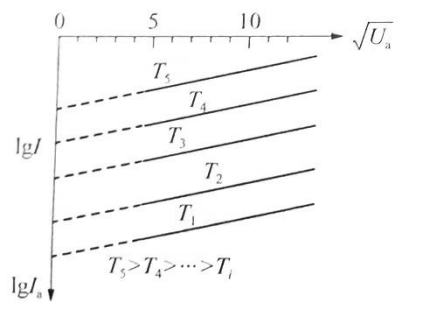
\includegraphics[clip,scale=1,trim={0 0 0 0}]{fig/fig8.png}
                     \caption{Extrapolation for zero-field currents}
                     \label{figure.8}
            \end{figure} 
   
   
	\section{Contents and Steps}
	\subsection{The Frank Hertz Experiment}
	Measurement of the first excitation potential of an atom. Through the $I_A\sim V_{G_2K}$ curve, the atomic energy quantization is observed and the first excitation potential of the dense atom is found. This electron tube synthesizer Frank-Hertz experiment module is divided into two modes: automatic and manual, where the experimental data obtained in the automatic mode can be reproduced on the oscilloscope after connecting the oscilloscope $I_A\sim V_{G_2K}$ curve.
	
	\subsubsection{Measured in automatic mode}
	\begin{itemize}
	\item connect the experimental circuit, power on.
	\item after the host is started, the main menu in the Frank Hertz experiment click on the "first column on the left" to set parameters, set the following parameters: filament voltage$V_f\approx 2.7V$, the first gate voltage $V_{G_1K}\approx 1.5V$, rejection voltage $V_{G_2K}\approx 9.0V$
	\item warm-up 3min, click the main menu of the Frank Hertz experiment "automatic mode", start the "automatic mode" experiment, the instrument control $V_{G_2K}$ from $0$ to $85V$ in $0.2V$ steps to draw $I_A\sim V_{G_2K}$ curve, and save the experimental data.
	\item Observe the curve form on the screen, if the curve cut the peak, should be appropriate to reduce the filament voltage $V_f$; if cut the valley, should be appropriate to reduce the rejection voltage $V_{G_2K}$. Restart until the $I_A\sim V_{G_2K}$curve including 6 intact peaks and valleys is drawn.
	\item In the main menu of Frank Hertz experiment, click "Next" on the right for data query. The most recent automatic mode measurement is listed on the screen, find each peak and valley of the current in the data list, and record the rejection voltage $V_{G_2K}$ corresponding to the extreme current in the table.
	\end{itemize}
    \subsubsection{Study the effect of each voltage on the  $I_A\sim V_{G_2K}$ curve}
    \begin{itemize}
    \item Effect of rejection voltage$V_{G_2A}$:
          \begin{itemize}
          \item Enter auto mode, set the filament voltage $V_f\approx 2.7V$, the first gate voltage $V_{G_1K}\approx 1.5V$, and the rejection voltage $V_{G_2K}\approx 6.0V$
          \item Draw the complete  $I_A\sim V_{G_2K}$ curve, return to the data query, record the peaks $V_{G_2K}$ and valleys corresponding to fill in the table.
          \item Adjust the rejection voltage $V_{G_2K}\approx 9.0V$, and repeat step 2.
          \item Analyze the changes in the peaks $V_{G_2K}$ and valleys of the curves at different rejection voltages and what are the patterns.
          \end{itemize}
    \item Effect of the first gate voltage:
          \begin{itemize}
          \item Set the filament voltage $V_f\approx 2.7V$, the first gate voltage $V_{G_1K}\approx 1.0V$, and the rejection voltage $V_{G_2K}\approx 9.0V$.
          \item Enter auto mode, click the "Auto $V_{G_2K}$" button, then start to draw the curve.
          \item After drawing the complete curve, set the first gate voltage $V_{G_1K}$ to $1.5V$ and start drawing the curve again. At this point, compare the difference between the previous curve and the new curve, and analyze how $V_{G_1K}$ affects the curve.
          \end{itemize}
    \item Effect of cathode filament voltage:
          \begin{itemize}
          \item Set the filament voltage $V_f\approx 2.7V$, the first gate voltage $V_{G_1K}\approx 1.5V$, and the rejection voltage $V_{G_2K}\approx 9.0V$.
          \item Enter auto mode, click the "Auto $V_{G_2K}$" button, and start to draw the curve.
          \item After drawing the complete curve, set the filament voltage $V_f$ to 2.7V and start drawing the curve again. Compare the difference between the two curves before and after, and analyze the influence of filament voltage $V_f$ on the curve.
          \end{itemize}
    \end{itemize}
    \subsection{Metal fugitive work experiment}
    \begin{itemize}
    \item Connect the experimental circuit and turn on the power. Adjust the ideal diode filament current A to be measured at $0.025A$ intervals between $0.6$ and $0.7A$. For each filament current, preheat for 3~5 min, corresponding to the temperature according to $T = 900+1430$ (if the anode current B is small or large, the filament current A can also be increased or decreased appropriately). For each filament current, add $36V,49V,64V,81V,100V,121V,144V$ to the anode in turn and fill in the table with the anode current of each group. 
    \item Note: When connecting the line before the start of the experiment and unplugging the line after the experiment, do not touch the metal part of the line to avoid high pressure on the body; because the experimental process may be in a long-term high pressure state, so the chassis temperature is high, the experimental data collection should be timely after the end of the pressure reduction or close the tester, while paying attention to cooling; experiments all electronic tube performance due to production reasons will not be completely consistent, so the same filament of different electronic tubes Current filament temperature may be different, so the value of the escaped electrons will not be identical. Multiple tubes can be used to calculate the average value of the experiment to reduce the error.
    \end{itemize}
    
    
	
	\section{Data processing}
	\subsection{The Frank Hertz Experiment}
	\subsubsection{Automatic mode measurements were recorded in the following table}
\begin{table}[htbp]
  \centering
  \caption{Automatic mode $I_A\sim V_{G_2K}$ Curve peak and valley voltage recording}
    \begin{tabular}{lrrrrrrrr}
    \toprule[2pt]
    Numble & 1     & 2     & 3     & 4     & 5     & \multicolumn{2}{c}{$V_{i+3}-V_i$} & \multicolumn{1}{l}{Mean} \\
    \midrule
    Peak $V_{G_2K}$ & 19.8  & 30.8  & 42.2  & 54.1  & 66.4  & 34.3  & 35.6  & 17.475 \\
    Valley $V_{G_2K}$ & 25.3  & 36.4  & 47.8  & 59.7  & 71.9  & 34.4  & 34.8  & 17.3 \\
  \bottomrule[2pt]
    \end{tabular}%
  \label{tab:addlabel}%
\end{table}%
From the peak and valley voltage values in the above table, the first excitation potential is calculated by the difference-by-difference method, and its average value is:
\begin{eqnarray}
\bar{V_0}=17.475 (V) 
\end{eqnarray}

\begin{figure}[H]
   \begin{minipage}[t]{0.5\linewidth}
      \centering
      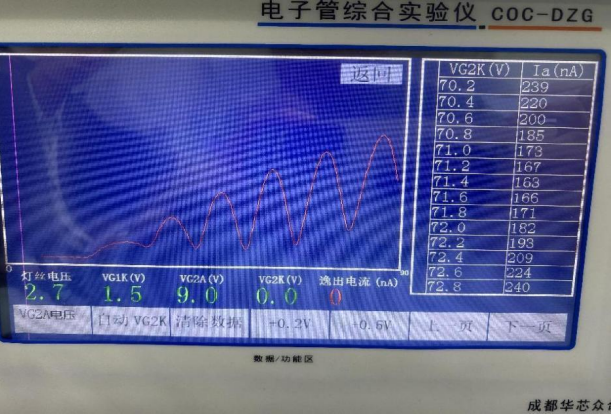
\includegraphics[clip,scale=1,trim={0 0 0 0}]{fig/fig9.png}
      \label{figure.9}
   \end{minipage}
   \begin{minipage}[t]{0.5\linewidth}
      \centering
      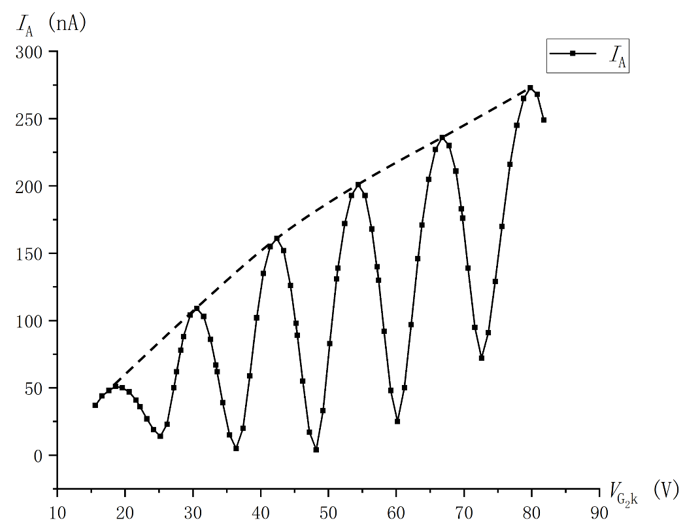
\includegraphics[clip,scale=0.8,trim={0 0 0 0}]{fig/fig10.png}
      \label{figure.10}
   \end{minipage}
   	  \caption{Automatic mode $I_A\sim V_{G_2K}$ Curve peak and valley voltage}
\end{figure} 

The relative error compared to the accepted value of the first excitation potential$U_0 = 11.55$ of the argon atom is:
\begin{eqnarray}
\left | (17.475-11.55)/11.55 \right | *100\% = 51.3\%
\end{eqnarray}

\subsubsection{The experimental data were recorded in the following table for changing each voltage on the $I_A\sim V_{G_2K}$ curve:}

A.Enter auto mode, set the filament voltage $V_f\approx 2.7V$, the first gate voltage $V_{G_1K}\approx 1.5V$, and the rejection voltage $V_{G_2K}\approx 6.0V$ curve is as follow:
\begin{figure}[H]
            	\centering
            	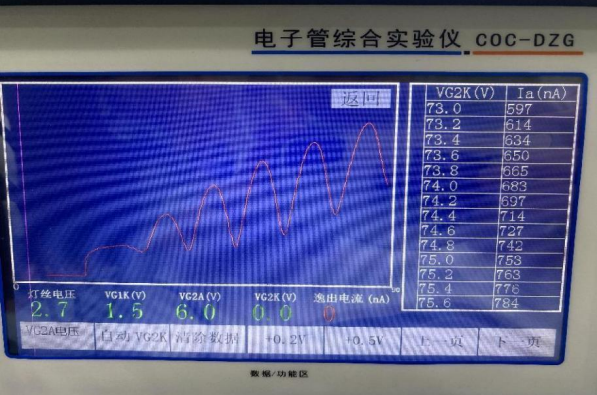
\includegraphics[clip,scale=0.8,trim={0 0 0 0}]{fig/fig11.png}
            	\caption{$I_A\sim V_{G_2K}$curve1}
            	\label{figure.11}
\end{figure}
The two images of the $I_A\sim V_{G_2K}$ curve were compared to observe the difference between the current intensity and the voltage change. It is easy to see that when the rejection voltage $V_{G_2K}$ decreases from $9.0V$ to $6.0V$, both the peaks and troughs of the images rise to some extent, while the overall image rises, which represents an increase in the overall current. The reason for this is as follows: the blocking effect of the gas atoms on the electrons is reduced, so the
electrons can easily pass through the energy level structure of the gas atoms, leading to an increase in the intensity of the current. At the same time, the electron energy increases and the speed increases, so the distance of electron movement in the tube increases. Therefore, when $V_{G_2K} =6.0V$, electrons easily pass through the energy level structure of the gas atoms, generating more current.

B.Set the filament voltage $V_f\approx 2.7V$, the first gate voltage $V_{G_1K}\approx 1.0V$, and the rejection voltage $V_{G_2K}\approx 9.0V$ curve is as follow:
\begin{figure}[H]
            	\centering
            	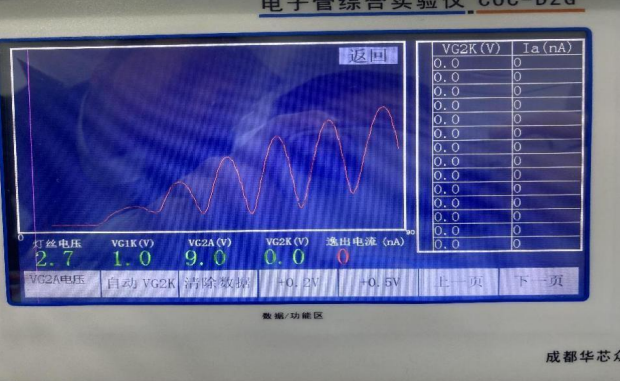
\includegraphics[clip,scale=0.8,trim={0 0 0 0}]{fig/fig12.png}
            	\caption{$I_A\sim V_{G_2K}$curve2}
            	\label{figure.12}
\end{figure}
When the first gate voltage $V_{G_1K}$ decreases from $1.5V$ to $1.0V$, the energy of electrons in passing through the first gate decreases and the speed of electrons decreases, so when $V_{G_1K}=1.0V$, the distance of electrons moving in the tube decreases, leading to a decrease in current intensity.Analysis of variability:
\begin{itemize}
\item Current intensity: When the first gate voltage $V_{G_1K}$ decreases from $1.5V$ to $1.0V$, the energy of electrons in passing through the first gate decreases and the speed decreases, leading to a decrease in current intensity. 
\item Change in the slope of the $I_A\sim V_{G_2K}$ curve: When the first gate voltage $V_{G_1K}$ decreases from $1.5V$ to$1.0V$, the slope of the $I_A\sim V_{G_2K}$ curve becomes smaller. This is because the decrease in the velocity of the electrons leads to a decrease in the distance the electrons move through the tube, and therefore the charge per unit time through the tube decreases, resulting in a slower rate of current with the increase in $V_{G_2K}$.
\end{itemize}

C.Set the filament voltage $V_f\approx 2.7V$, the first gate voltage $V_{G_1K}\approx 1.5V$, and the rejection voltage $V_{G_2K}\approx 9.0V$ curve is as follow:
\begin{figure}[H]
            	\centering
            	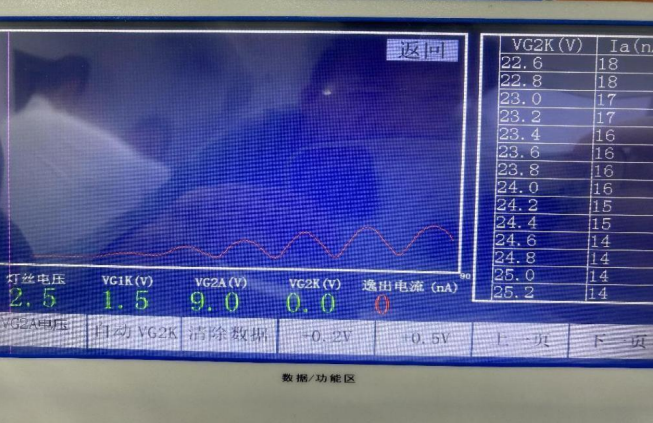
\includegraphics[clip,scale=0.8,trim={0 0 0 0}]{fig/fig13.png}
            	\caption{$I_A\sim V_{G_2K}$curve3}
            	\label{figure.13}
\end{figure}
When the filament voltage $V_f$ is reduced from $2.7 V$ to $2.5 V$, the energy of the heated filament will be reduced, resulting in poorer electron emission and reduced current intensity. Variance analysis:

\begin{itemize}
\item Current intensity: When the filament voltage$V_f$ decreases from $2.7V$ to $2.5V$, the electron emission ability becomes worse and the current intensity decreases.
\item Shape of $I_A\sim V_{G_2K}$ curve: When the filament voltage $V_f$ decreases from $2.7V$ to $2.5V$, the electron emission ability becomes worse, so the slope of the $I_A\sim V_{G_2K}$ curve becomes smaller and the rising part of the curve becomes flatter.
\end{itemize}

Conclusion:Filament voltage is a key factor affecting the cathode's ability to emit electrons, so its variation may have a more significant effect on the $I_A\sim V_{G_2K}$ curve. In the Frank Hertz experiment, the change of filament voltage changes the number and energy of cathode emitted electrons, which affects the current intensity and the shape of the $I_A\sim V_{G_2K}$ curve. Also,changes in the rejection voltage $V_{G_2K}$ and the first gate voltage $V_{G_1K}$ directly affect the electron movement in the tube and have a significant effect on the $I_A\sim V_{G_2K}$ curve. Therefore, we need to consider the effects of these variables on the $I_A\sim V_{G_2K}$ curve together.
\subsection{Metal fugitive work experiment}
\subsubsection{Record the experimental data in the following table}
Anode current values $I_a$ corresponding to different filament currents $I_F$ and anode voltages $U_a$
\begin{table}[htbp]
  \centering
    \begin{tabular}{lrrrrrrr}
        \toprule[2pt]
    $U_a/I_F$ & \multicolumn{1}{l}{16V} & \multicolumn{1}{l}{25V} & \multicolumn{1}{l}{36V} & \multicolumn{1}{l}{49V} & \multicolumn{1}{l}{64V} & \multicolumn{1}{l}{81V} & \multicolumn{1}{l}{100V} \\
        \midrule
    0.600A & 0.064 & 0.067 & 0.071 & 0.073 & 0.075 & 0.079 & 0.081 \\
    0.625A & 0.117 & 0.125 & 0.131 & 0.136 & 0.142 & 0.145 & 0.149 \\
    0.650A & 0.211 & 0.225 & 0.236 & 0.246 & 0.254 & 0.260  & 0.268 \\
    0.675A & 0.361 & 0.391 & 0.409 & 0.429 & 0.440  & 0.451 & 0.465 \\
    0.700A & 0.589 & 0.644 & 0.681 & 0.714 & 0.734 & 0.761 & 0.779 \\
      \bottomrule[2pt]
    \end{tabular}%
  \label{tab:addlabel}%
\end{table}%

$\lg_{}{I_a}-\sqrt{U_a}$ graph line is made from the data in the table. The intercept $\lg{I_a}=\lg{I}+\frac{0.439\sqrt{E_a} }{2.30T}  $of the straight line is $\lg{I}$ in Eq. From this, the zero-field hot electron emission current $I$ at different cathode temperatures is obtained.
\begin{figure}[H]
            	\centering
            	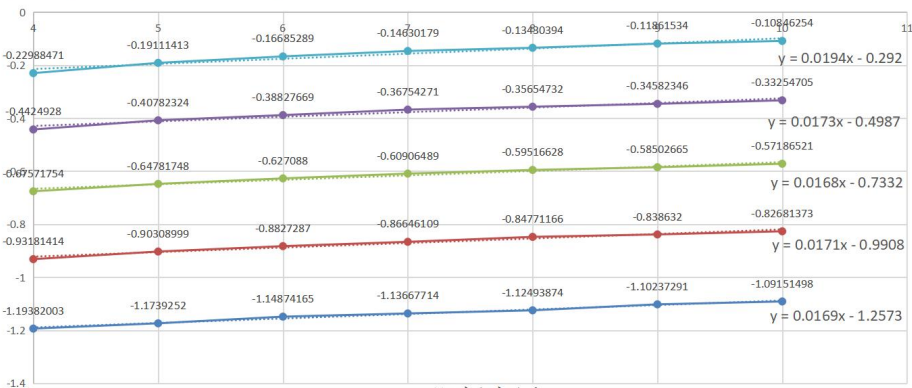
\includegraphics[clip,scale=1,trim={0 0 0 0}]{fig/fig14.png}
            	\caption{Anode current values for different filament currents and anode voltages}
            	\label{figure.14}
\end{figure}
Processing the data from the graphs gives:
\begin{eqnarray}
\begin{cases}
 \lg I_1 = -1.2573mA\\
 \lg I_2 = -0.9908mA\\
 \lg I_3 = -0.7332mA\\
 \lg I_4 = -0.4987mA\\
 \lg I_5 = -0.2920mA
\end{cases}\qquad \Longrightarrow \qquad \begin{cases}
 I_1=0.0169\\
 I_2=0.0171\\
 I_3=0.0168\\
 I_4=0.0173\\
 I_5=0.0194
\end{cases}
\end{eqnarray}

Fill in the following table with the intercepts of the lines at each temperature of the above graph to make  $\lg{\frac{1}{T^2}\sim \frac{1}{T} } $  graph line.
\begin{table}[htbp]
  \centering
    \begin{tabular}{rrrrr}
    \toprule[2pt]
    \multicolumn{1}{l}{$I_F/A$} & \multicolumn{1}{l}{$T/K$} & \multicolumn{1}{l}{$\lg I /mA$} & \multicolumn{1}{l}{$1/T$} & \multicolumn{1}{l}{$\lg \frac {1}{T\^2}$} \\
    \midrule
    0.600   & 1758.00  & -1.2573 & 5.69  & -7.851 \\
    0.625 & 1793.75 & -0.9908 & 5.58  & -7.521 \\
    0.650  & 1829.50 & -0.7332 & 5.47  & -7.237 \\
    0.675 & 1865.25 & -0.4987 & 5.36  & -7.006 \\
    0.700   & 1901.00  & -0.2920 & 5.26  & -6.811 \\
    \bottomrule[2pt]
    \end{tabular}%
  \label{tab:addlabel}%
\end{table}%
\begin{figure}[H]
            	\centering
            	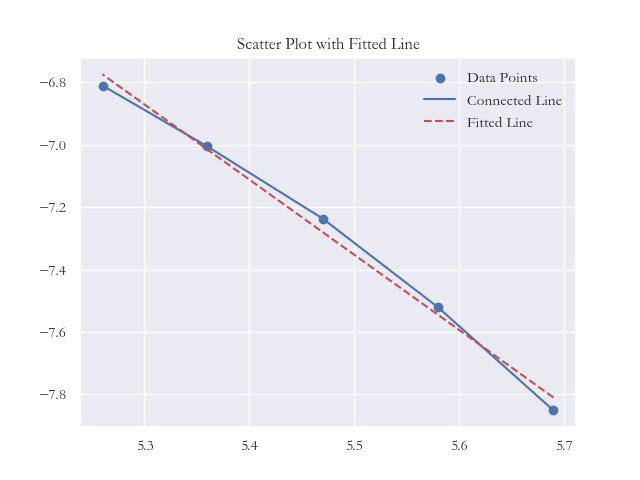
\includegraphics[clip,scale=1,trim={0 0 0 0}]{fig/fig15.png}
            	\caption{Scatter Plot with Fitted Line}
            	\label{figure.15}
\end{figure}
The line is:
\begin{eqnarray}
y = -2.4084x + 5.8937 \qquad (R^2=0.992)
\end{eqnarray}

According to the slope of the straight line of :
\begin{eqnarray}
\lg{\frac{1}{T^2} } \sim \frac{1}{T} = -2.4084
\end{eqnarray}

substitute into :
\begin{eqnarray}
\lg \frac{I}{T^{2}}=\lg A S-\frac{e \varphi}{2.30 k T}=\lg A S-5.04 * 10^{3} \varphi \frac{1}{T}
\end{eqnarray}

The electron escape work of tungsten metal is found to be:
\begin{eqnarray}
4.78eV
\end{eqnarray}

and compared with the accepted value of 4.54 eV, and the value obtained by calculating the relative error is:
\begin{eqnarray}
|4.78-4.54| / 4.54 \times 100 \% \approx 5.29 \%
\end{eqnarray}


\section{Conclusion and analysis}
\subsection{The Frank Hertz Experiment}
Through data processing, the study -curve periodic peaks and valleys yielded the first excitation potential of the argon atom: $17.475V$, and proved the existence of the atomic energy level. The factors that affect the anode current of the inflatable electron tube are: filament voltage, first gate voltage and rejection voltage.
\begin{itemize}
\item \textbf{Why $I_A \sim V_{G_2K}$ does the curve change periodically?}\\
It is fundamentally due to the presence of atomic energy levels. In experiments, when the voltage increases, electrons have higher energy and are able to leap to higher energy levels. When the voltage reaches a certain value, the electrons can jump to the next energy level, which leads to a sudden increase in current. When the voltage continues to increase, the electrons continue to acquire higher energy and can leap to higher energy levels, but the energy difference between these levels is different, thus leading to a decrease in the current between the peaks. Thus a periodic variation is observed.
\item \textbf{How should I adjust the $I_A \sim V_{G_2K}$ curve if it is clipping? If there is a trough, how should it be adjusted?}\\
If the I-V curve is clipping, reduce the filament voltage/first gate voltage or increase the rejection voltage. The opposite is true for valley clippvoltage.ing: increase the filament voltage/first gate voltage or decrease the rejection voltage.
\item \textbf{What is the ef ect of changing the filament voltage $V_f$, the first gate voltage $V_{G_1K}$, and the
rejection voltage $V_{G_2K}$, respective to $I_A \sim V_{G_2K}$?}\\
Filament voltage: increase: increase the current peak and average value; decrease: decrease the current peak and average value. First gate voltage: increase: increase the current peak and average value; decrease: decrease the current peak and average value. Rejection voltage: Decrease: Increase current peak and average value; Increase: Decrease current peak and average value
\end{itemize} 

\subsection{Metal fugitive work experiment}
The work of escape of metallic tungsten measured by the Richardson linear method was $4.78eV$. This indicates that the energy required for the escape of electrons from the surface of the metal is high and that this is related to the physical and chemical properties of the metal.
\begin{itemize}
\item \textbf{What are the advantages of the Richardson Straight Line Method?}\\
High accuracy: compared with other fugitive work measurement methods, more accurate fugitive work values can be obtained; easy experiment: only the current magnitude of the metal at different temperatures needs to be measured, and then data processing can be performed to obtain the fugitive work values.
\item \textbf{What is fugitive work? Is fugitive work?}\\
The work of escape is the minimum energy required for an electron to escape from a solid material. The nucleus of the same metal has the same binding capacity for the electrons outside the nucleus, so it does the same work for the electrons outside the nucleus to escape, so the work of escape is certain.
\end{itemize}

\begin{appendix}
	\section{Data Analysis and Visualisation Source Code}
	\begin{lstlisting}[language=python]
import scipy.stats as st
import seaborn as sns
import pandas as pd
import numpy as np
from matplotlib import pyplot as plt
from scipy.optimize import curve_fit#拟合
#=======================================
#图片背景设置
plt.style.use('seaborn-darkgrid')
sns.set(style = 'darkgrid')
import  warnings
warnings.filterwarnings('ignore')
plt.rcParams['font.sans-serif'] = ['STSong']

x = np.array([5.69,5.58,5.47,5.36,5.26])  # 第一列数据
y = np.array([-7.851,-7.521,-7.237,-7.006,-6.811])  # 第二列数据

# 绘制散点图
plt.scatter(x, y, label='Data Points')

# 连线
plt.plot(x, y, label='Connected Line')

# 拟合直线
fit = np.polyfit(x, y, 1)  # 一阶多项式拟合
fit_fn = np.poly1d(fit)
plt.plot(x, fit_fn(x), '--r', label='Fitted Line')

# 设置图例和标题
plt.legend()
plt.title('Scatter Plot with Fitted Line')

# 显示图形
plt.show()
	\end{lstlisting}
\section{Related photo records}
\begin{figure}[H]
            	\centering
            	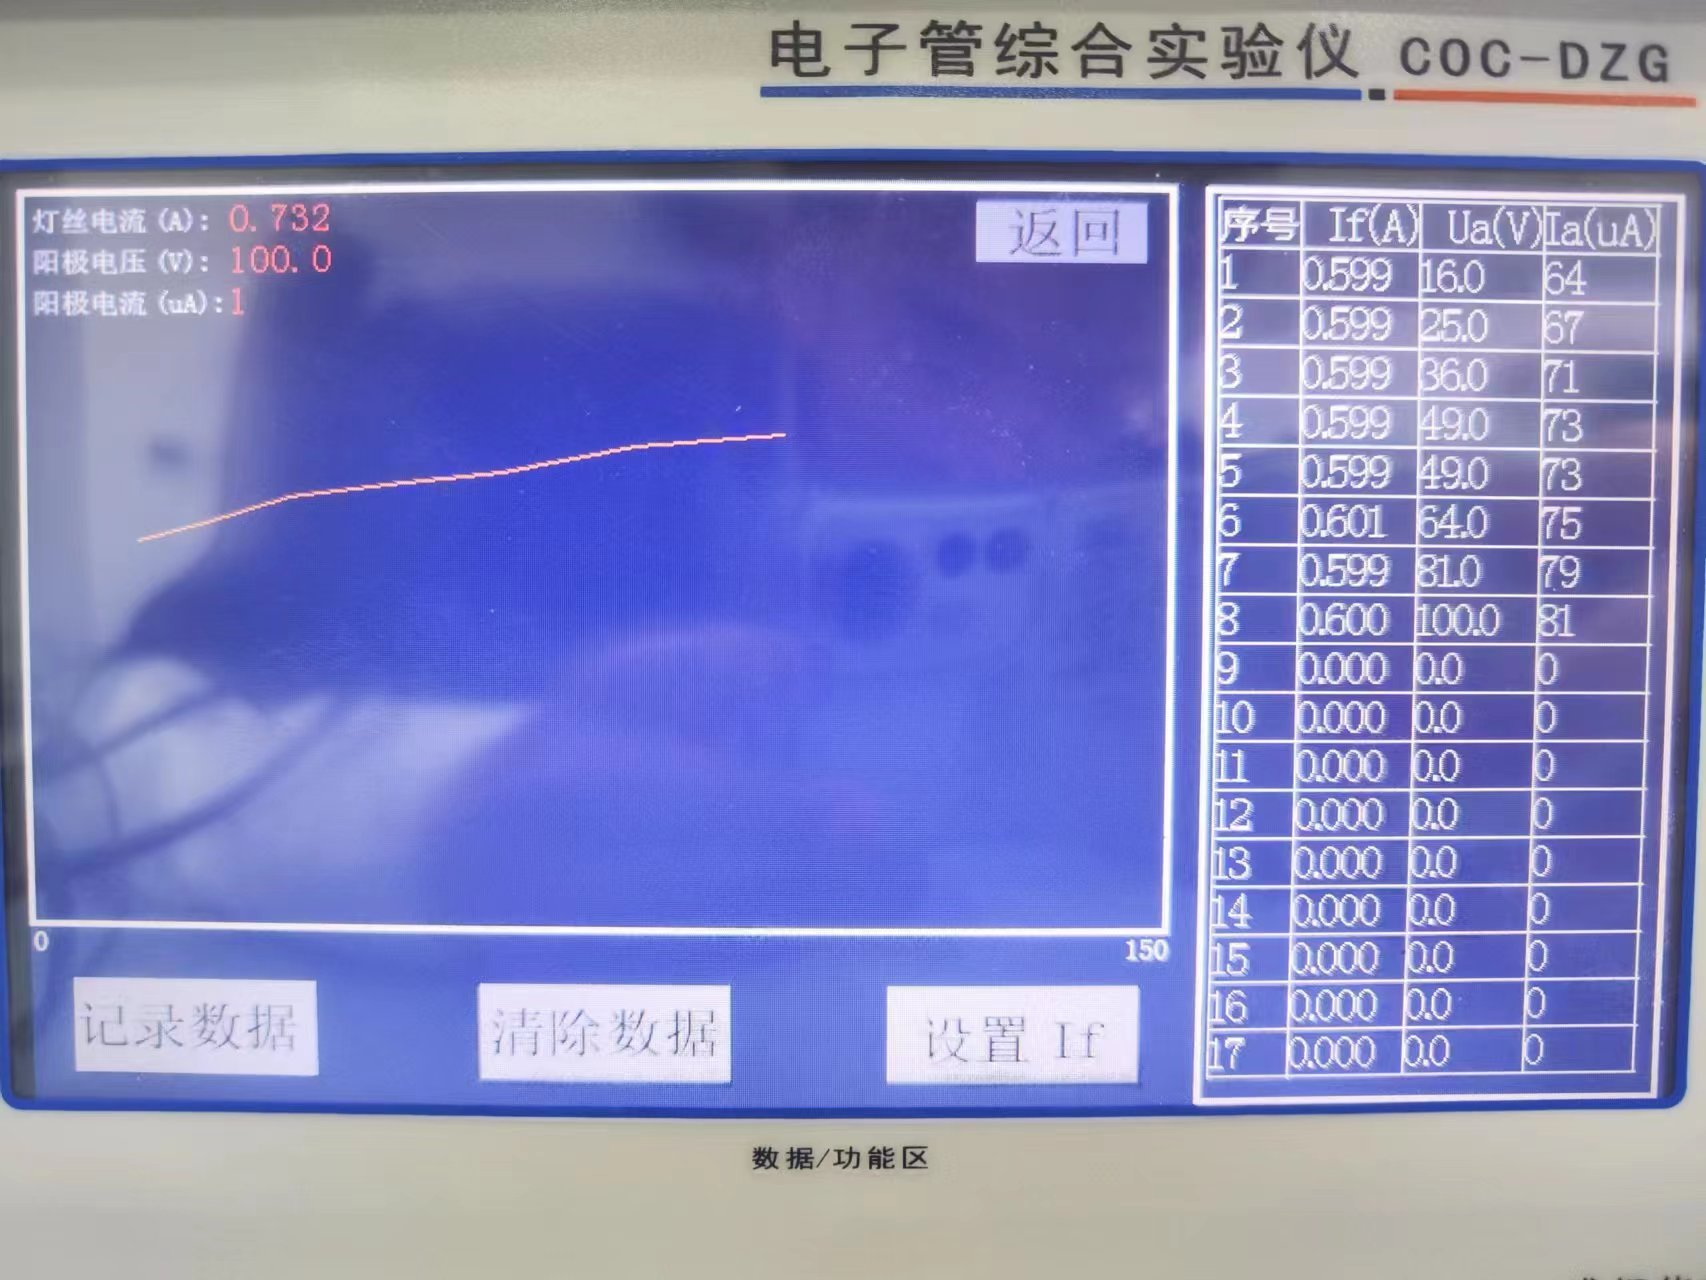
\includegraphics[clip,scale=0.2,trim={0 0 0 0}]{fig/fig16.jpg}
            	\label{figure.16}
\end{figure}
\begin{figure}[H]
            	\centering
            	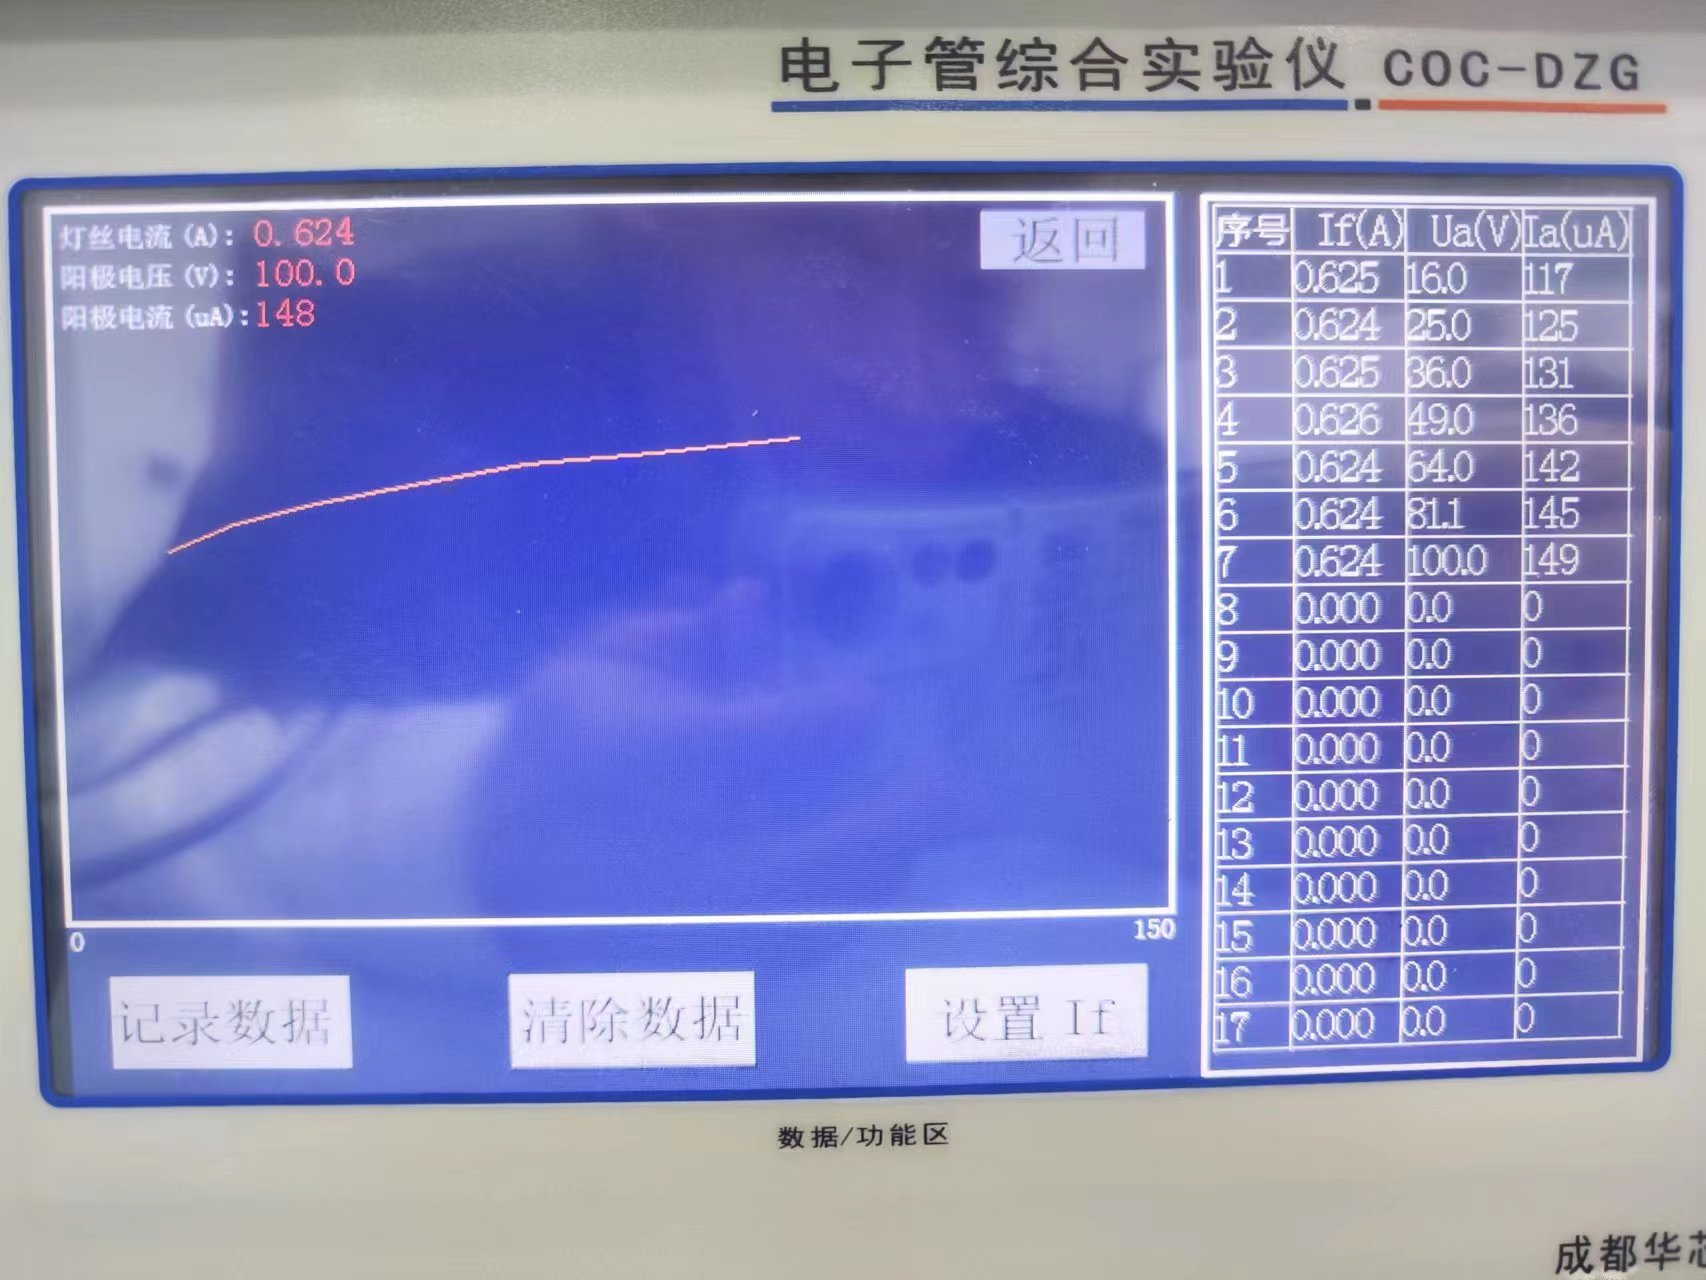
\includegraphics[clip,scale=0.2,trim={0 0 0 0}]{fig/fig17.jpg}
            	\label{figure.15}
\end{figure}
\begin{figure}[H]
            	\centering
            	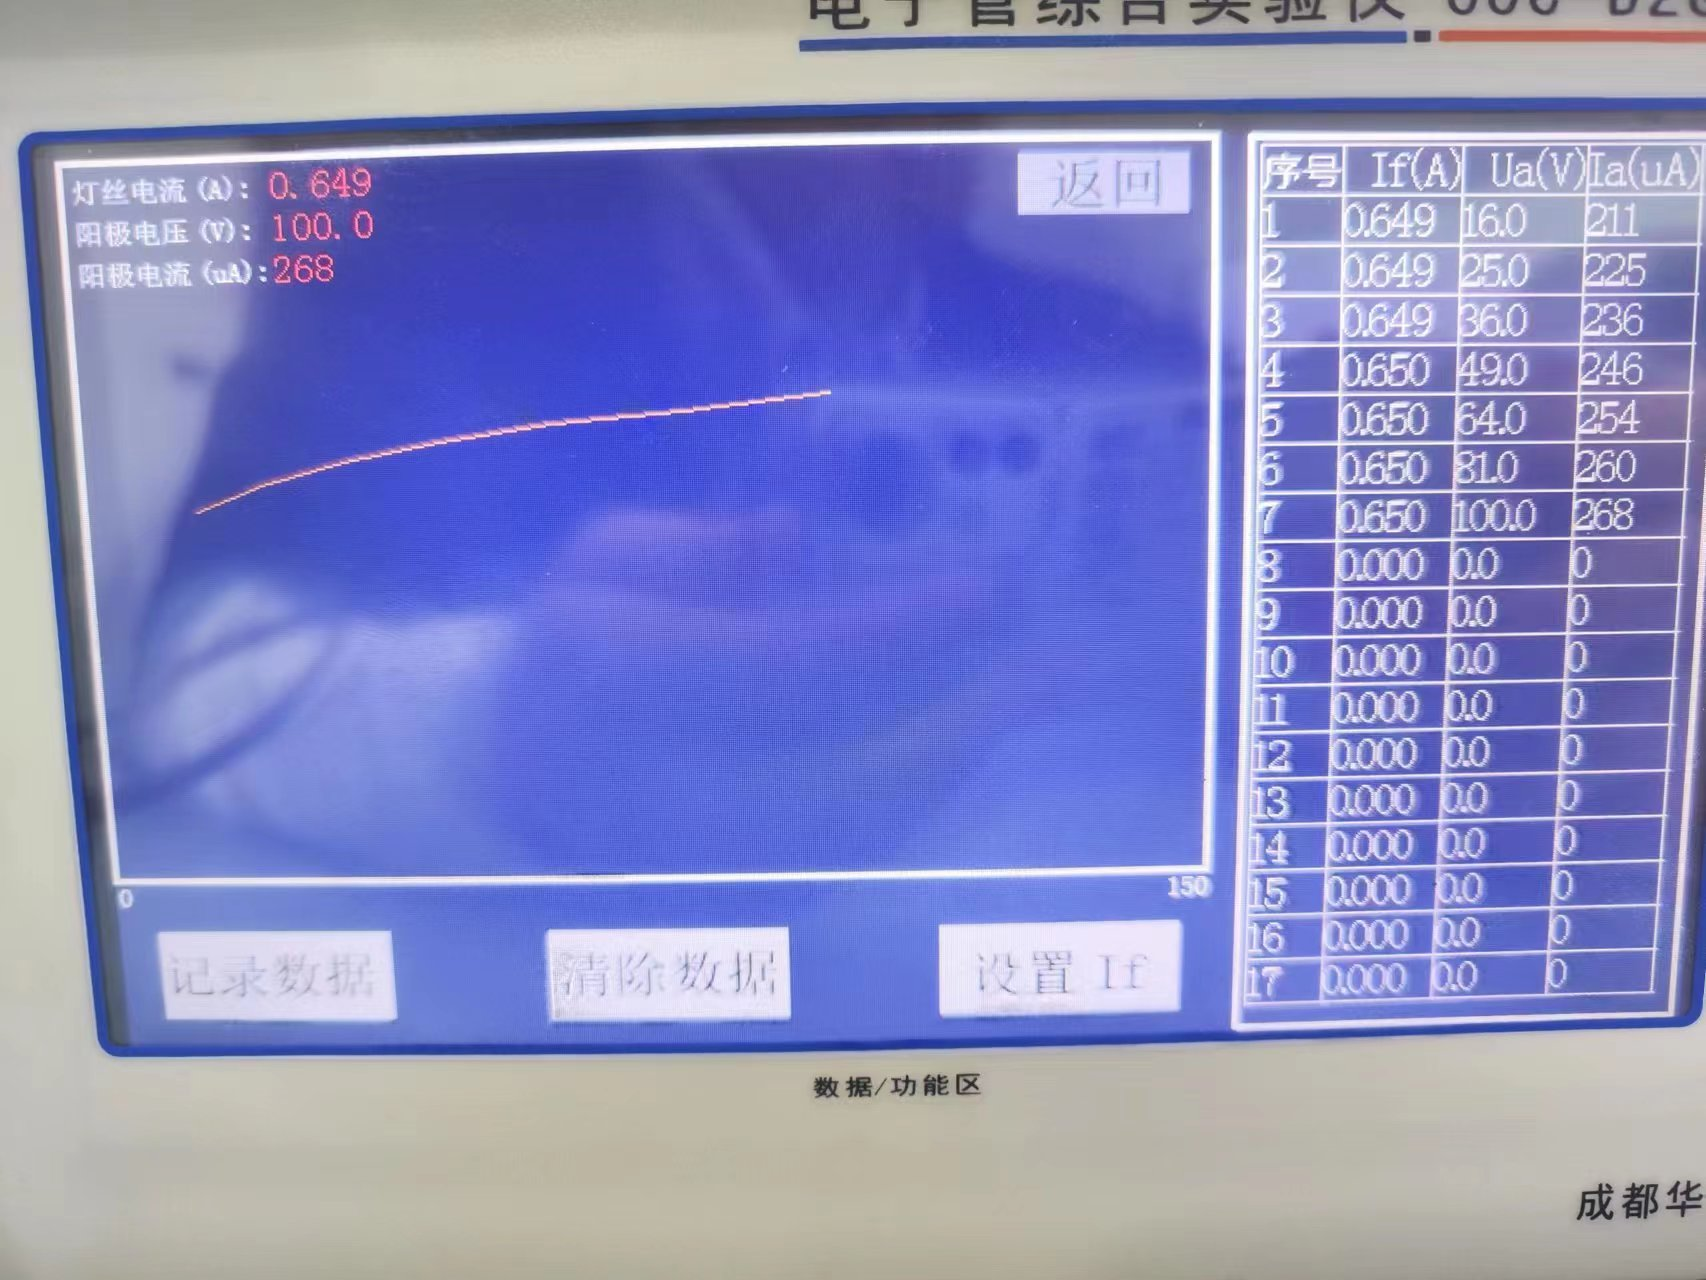
\includegraphics[clip,scale=0.2,trim={0 0 0 0}]{fig/fig18.jpg}
            	\label{figure.15}
\end{figure}
\begin{figure}[H]
            	\centering
            	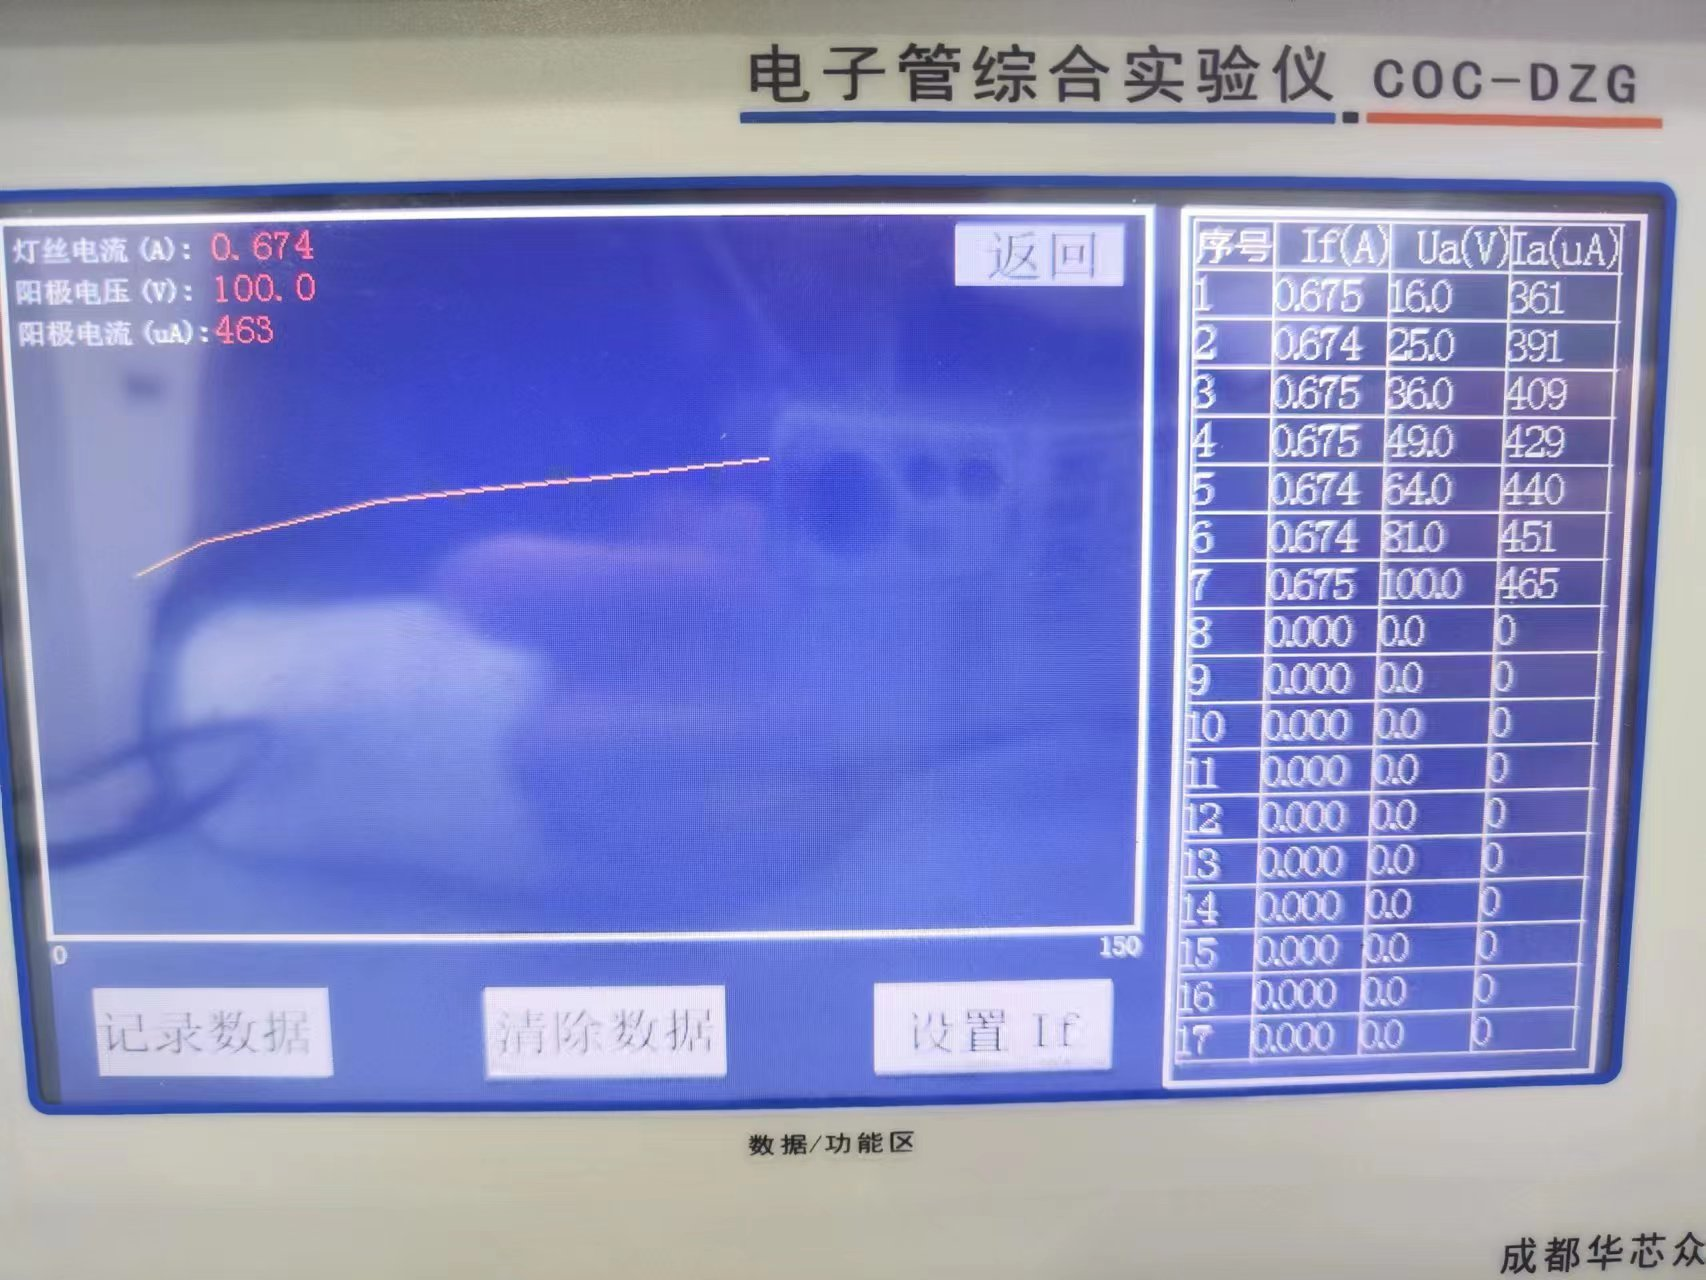
\includegraphics[clip,scale=0.2,trim={0 0 0 0}]{fig/fig19.jpg}
            	\label{figure.15}
\end{figure}
\begin{figure}[H]
            	\centering
            	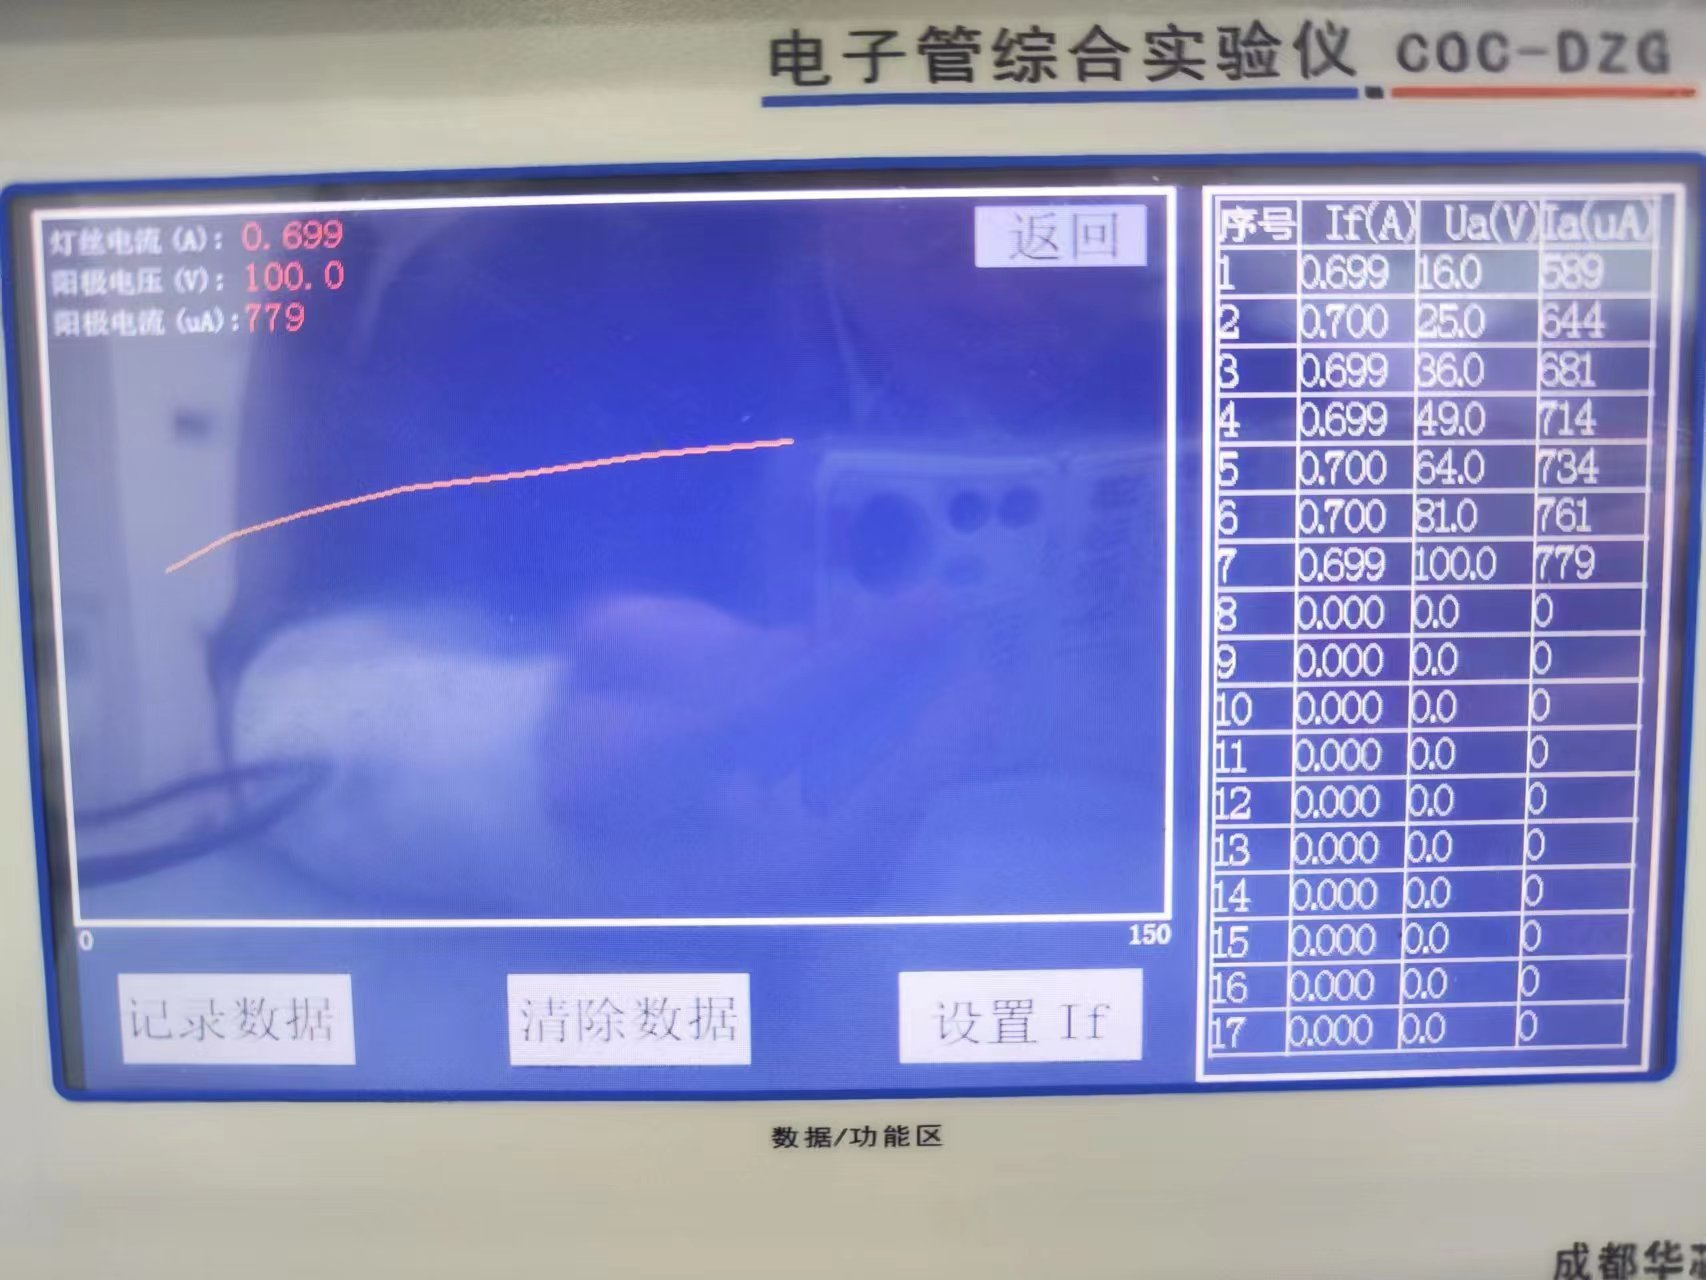
\includegraphics[clip,scale=0.2,trim={0 0 0 0}]{fig/fig20.jpg}
            	\label{figure.15}
\end{figure}


\end{appendix}


\end{document}  